\QAUappendixsetup
\chapter{补充试验数据与说明}\label{app:appendixA}

本附录用于放置不便纳入正文、但对理解研究过程与结果具有辅助价值的补充材料，例如原始测定项目列表、补充图表、参数设定说明、缩略语说明及统计分析补充结果等。附录内容的编排原则应与正文保持一致，文字说明采用宋体小四，图题表题格式与正文相同。

\section{缩略语说明示例}

\begin{center}
	\captionof{table}[研究中常用缩略语示例]{研究中常用缩略语示例\par
		{\qauTimes\fontsize{10.5bp}{15.75bp}\selectfont \textbf{Table~\thetable\ Examples of common abbreviations used in this study}}}
	\label{tab:appendix-abbr}
	\renewcommand{\arraystretch}{1.5}
	{\songti\zihao{5}
		\begin{tabular*}{0.8\textwidth}{@{\extracolsep{\fill}}>{\centering\arraybackslash}m{0.20\textwidth}>{\centering\arraybackslash}m{0.50\textwidth}}
			\toprule
			缩略语 & 含义 \\
			\midrule
			AA & 抗坏血酸 (Ascorbic acid) \\
			BI & 褐变指数 (Browning index) \\
			PPO & 多酚氧化酶 (Polyphenol oxidase) \\
			POD & 过氧化物酶 (Peroxidase) \\
			\bottomrule
		\end{tabular*}
	}
\end{center}

\section{补充图表示例}

\begin{center}
	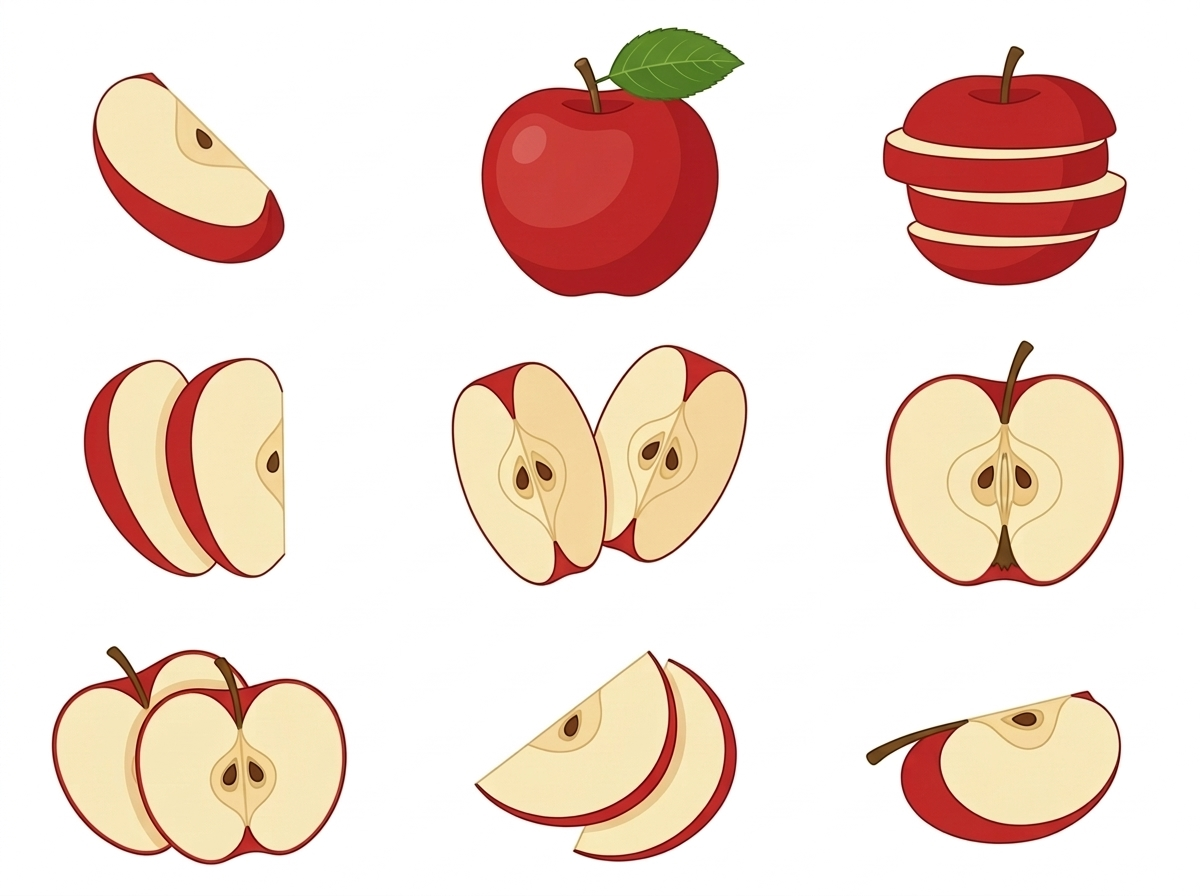
\includegraphics[width=0.45\textwidth]{figures/apple.png}
    \captionof{figure}[附录 A 中补充图片占位示例]{附录 A 中补充图片占位示例。\par
	（A）XXXX；（B）XXXX；（C）XXXX。\par
	注：不同小写字母代表存在显著差异（$p<0.05$）。\par
	{\qauTimes\fontsize{10.5bp}{15.75bp}\selectfont \textbf{Fig.~\thefigure\ Example of supplementary figure in Appendix B.}}\par
	{\qauTimes\fontsize{10.5bp}{15.75bp}\selectfont \textbf{(A) XXXX; (B) XXXX; (C) XXXX.}}\par
    {\qauTimes\fontsize{10.5bp}{15.75bp}\selectfont \textbf{Different lowercase letters indicate significant differences (\boldmath$p<0.05$).}}}
	\label{fig:appendix-layer}
\end{center}

附录中的图表仍建议按照所在附录章节顺序连续编号，并在正文中首次引用相关附录时给出明确指引，例如“详见附录 A 中表 A.1”。